\chapter{Causal Inference Based Fault Localization for Numerical Software with Bayesian Additive Regression Trees}\label{chap:BART}


\section{Introduction}\label{BARTintro}
\vspace{-2pt}
In causal inference based SFL techniques\cite{bai2015numfl, baah2010causal, baah2011mitigating,shu2013mfl}, fault localization method basically contains two steps: (1) controlling the confounding bias which is caused by confounding variables. (2) estimating average failure causing effect of treatment variable $T$ on outcome $Y$. Here, the second step, AFCE estimation, is a challenging work because the functional form of the relationship between $T$ and $Y$ are unknown. The previous work, Baah et al’s causal estimator estimate AFCE with parametric regression model, which requires pre-defined of the functional form of the dose response function of treatment $T$ (e.g. NUMFL has pre-defined DRF curve as shown in Figure 3.4 ). But if the parametric model is misspecified, the AFCE estimation can be biased.

To solve the above problem, a non-parametric causal effect estimation model called Bayesian Additive Regression Trees(BART) has been proposed by Hill et al \cite{hill2012bayesian}. BART use a sum of trees structure to approximate the dose response function (DRF) of both the treatment variable and the confounding variables. 
Comparing to methods such as NUMFL and Baah et al’s causal estimator, BART requires less guess-work in modeling dose response function.   

In this chapter, we proposal a new statistical fault localization method based on BART model and evaluate it on numerical programs with single or multiple faults. The motivation for using BART in statistical fault localization is:
\vspace{-0.2cm}
\begin{itemize}
\item BART can flexibly fit non-linear response surfaces even with a large number of predictors
\item BART does not require the researcher to specify the functional form of the relationship between treatment and outcome. The user only need to input the treatment, confounding variable and the outcome, but not need to provide how these variables are parametrically related. Also, comparing to NUMFL, BART does not require a separate step to control confounding bias.
\item BART has been proved to be more effective than propensity score matching based causal inference methods in average causal effect estimation for binary treatment. It also has potential in estimating unbiased average causal effect for continuous treatment \cite{hill2012bayesian, hill2013assessing}.
\item BART algorithm software is freely available and easy to use \cite{BARTMachine}.
\end{itemize}

The rest of the chapter is organized as follows: we present the background of single regression tree and BART model in Section \ref{BARTbg}; Using BART model to estimate failure-causing effect is described in detail in Section \ref{BARTafce};  we report the empirical evaluation in Section \ref{BARTevaluation}; related work is surveyed in Section \ref{BARTrelatedwork}; and Section \ref{BARTconclusion} concludes the chapter.

\section{BART Model Algorithm}\label{BARTbg}%what is BART and why BART
The BART model algorithm consists of three parts: a sum of regression trees model, a regularization prior and a fitting algorithm, Marcov Chain Mote Carlo (MCMC)
\subsection{A Single Regression Tree model}
Regression tree is one type of decision tree that predicts the value of a target variable based on several input variables \cite{loh2011classification}. Regression tree handles the situation when the target variable is continuous. Figure \ref{singlergt} shows a single regression tree model. All the interior nodes of a regression tree have decision rules which send the input data set to either left or right side. After the input data set go through the interior nodes and reach the bottom of the tree, the data set is divided into several disjoint subgroup. Each group of data is represent by a leaf node.

\begin{figure*}[!thpb]
\centering
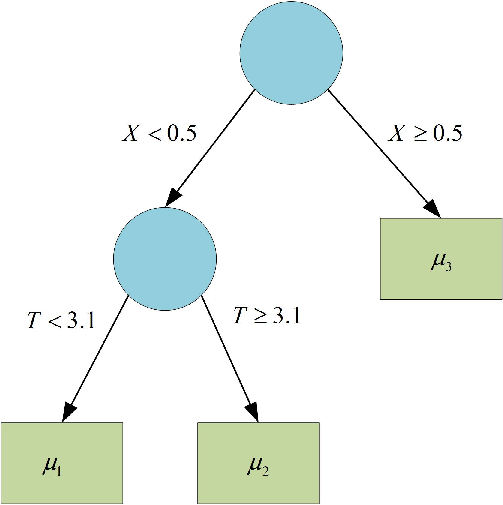
\includegraphics[width=0.5\textwidth]{chapter4_SingleRGT.pdf}
\caption{Single Regression Tree Structure}
\label{singlergt}
\end{figure*}

A single regression tree model is denoted as:
\begin{equation*}
Y=g(\pmb{Z}; R, M)+\epsilon
\end{equation*}
Here $\varepsilon  \sim N(0,{\sigma ^2})$ is a normal distributed error. $\pmb{Z}=[T,\pmb{X}]$ denotes all the variables related to the outcome $Y$, so $Z$ includes both treatment variable $T$ and confounding variables $\pmb{X}$. $R$ denotes a binary regression tree consisting a set of interior node decision rules and a set of terminal nodes, and let $M=
\begin{Bmatrix}
 \mu _1, \mu _2, . . ., \mu _b
\end{Bmatrix}$
denotes a set of parameter value associated with each of the $b$ terminal nodes of $R$. Each terminal node represent a regression model of outcome $Y$ on all the variables $Z$.

A regression tree model is often used in approximating unknown functions. For example, the dose response function of the treatment variable, $Y=f(T,\pmb{X})$. The regression tree model divides the value space of $[T,\pmb{X}]$ in to several subgroups with its tree structure and fit a regression model for each subgroup. When making inference of $Y$ given a specific unit of treatment and confounding variables values $[T=t,\pmb{X}=\pmb{x}]$, the regression will first find out which subgroup the unit belongs to and then infer outcome $Y$ with the corresponding linear regression. Regression tree model has two advantages: (1) making prediction is fast. (2) it can handle non-linear function approximation.


\subsection{A sum of regression trees model}
BART model is a sum of trees model. With the definition of a single tree model, the sum of trees model can be expressed as:
\begin{equation*}
Y = g(\pmb{Z};{R_1},{M_1}) + g(\pmb{Z};{R_1},{M_1}) +  \cdots  + g(\pmb{Z};{R_m},{M_m}) + \varepsilon
\end{equation*}
where each $(R_i,M_i)$ denotes a single sub-tree model and $\varepsilon  \sim N(0,{\sigma ^2})$.  $m$ denotes the number of trees in BART model. We have
 \begin{equation*}
 Y =f(\pmb{Z})=f(T,\pmb{X})= \left( {\sum\limits_{j = 1}^m {g(T,\pmb{X};{R_j},{M_j})} } \right) + \varepsilon
 \end{equation*}

Comparing to single regression tree model, BART model has two advantages. First BART can incorporate interaction effects of varying orders. Unlike the single tree model, when $m>1$ the terminal node $\mu_i$ given by $g(\pmb{Z};{R_i},{M_i})$ is merely part of the conditional mean of $Y$ given $Z$. If the assignment of $\mu_i$ depends on just a single component of $Z$ (only one variable),  $\mu_i$  represents direct effect of that variable to $Y$. If the assignment of $\mu_i$ depends on more than one component of $Z$ (e.g., more than one variable), the terminal node will represent interaction effects of those variables. Because the BART model may be based on trees of varying sizes, the sum of trees structure can incorporate both direct effects and interaction effects of varying orders \cite{conference1997advances}. Second, fitting BART model does not has much more computation cost than fitting a large single tree model. This is because that BART can scale to large datasets using a parallel MCMC sampler \cite{pratola2014parallel, pratola2015bayesian}.  

\subsection{A regularization prior}
Fitting the BART model requires a prior of all the parameters of the sum of trees model.  The prior regularize the fit by keeping the individual tree's effect from being unduly influential. Without such a prior, large  tee components would dominate the sum of trees structure. The regularization prior can also help BART avoid overfitting. To simplify the prior specification, the trees in BART model $(R_1, M_1), (R_2,M_2), \ldots, (R_m, M_m) $ are considered to be independent of each other and of $\sigma$. Also, the terminal node parameters $ \mu _{1j}, \mu _{2j}, . . ., \mu _{bj} $ of every tree $R_j$ are independent. So we have:

\begin{equation*}
 \begin{array}{l}
P(({R_1},{M_1}),({R_2},{M_2}) \ldots ,({R_m},{M_m}),\sigma ) = \left[ {\prod\limits_j {P({R_j},{M_j})} } \right]p(\sigma )\\
\quad \quad \quad \quad \quad \quad \quad \quad \quad \quad \quad \quad \quad \quad \; = \left[ {\prod\limits_j {P({M_j}|{R_j})P({R_j})} } \right]p(\sigma )
\end{array}
 \end{equation*}
and
\begin{equation*}
P({M_j}|{R_j}) = \left[ {\prod\limits_i {P({\mu _{ij}}|{R_j})} } \right]
 \end{equation*}
Here ${\mu _{ij}} \in {M_j}$ denotes the $ith$ terminal node of the $jth$ regression tree From the above equations, we can see the independence simplify the prior specification problem to the specification of prior for just ${P({\mu _{ij}}|{R_j})}$, $P({R_j})$ and $P(\sigma)$. In \cite{chipman2010bart}, the specification of prior forms on $P(\sigma)$ is defined as the inverse chi-square distribution. The prior on ${P({\mu _{ij}}|{R_j})}$ is defined as conjugate normal distribution. The prior on $P(R_j)$ is complicated which contains 3 aspects:
\begin{enumerate}
\item the probability that a nonterminal node at depth $d$ is given by
\begin{equation*}
\alpha {(1 + d)^{ - \beta }},\quad \alpha  \in (0,1),\beta  \in [0,\infty )
 \end{equation*}
\item the prior probability that a variable is selected as the splitting variable at an interior node is $1/k$ and $k$ is the total number of variables including both treatment and confounders.
\item the prior probability that a splitting variable split at value $x$ is $1/N$ and $N$ is the total number of observed values of the splitting variable in the sample data set.
\end{enumerate}
The detail of the prior specification for ${P({\mu _{ij}}|{R_j})}$, $P({R_j})$ and $P(\sigma)$ can be reffered to \cite{chipman2010bart}.


\subsection{Bayesian Backfitting MCMC Algorithm}
BART uses a Bayesian backfitting  MCMC algorithm to fit the model \cite{gilks2005markov}. The algorithm uses Gibbs sampler \cite{casella1992explaining}. The Gibbs sampler get $m$ successive draws of $(R_j, M_j)$ conditionally on $(R_{(j)}, M_{(j)}, \sigma)$:

\begin{equation*}
(R_j,M_j)|R_{(j)}, M_{(j)}, \sigma, Y
\end{equation*}
$j=1 \ldots m$, followed by a draw of $\sigma$ from the full conditional:

\begin{equation*}
\sigma |{R_1}, \ldots ,{R_m},{M_1}, \ldots ,{M_m},Y
\end{equation*}
Here $R_{(j)}$ represents all the trees except $R_j$, so $R_{(j)}$ will be a set of $m-1$ trees. $M_{(j)}$ is similarly defined as $R_{(j)}$.

\section{AFCE Estimation With BART}\label{BARTafce}% how to use BART

In this section, we introduce the method of using BART to estimate failure-causing effect of a numerical expression. Hill et al. have proved that BART is effective in average causal effect estimation when the treatment variable is binary. Here, we first briefly reviewed Hill’s algorithm:

If the treatment variable is binary, BART model primarily estimate failure-causing effects such as $E(Y(1)|\pmb{X}=\pmb{x}) - E(Y(0)|\pmb{X}=\pmb{x})=E(Y|T=1, \pmb{X}=\pmb{x})-E(Y|T=0, \pmb{X}=\pmb{x})=f(1,\pmb(x))-f(0,\pmb(x))$ . The algorithm contains the following steps:
\begin{enumerate}
\item Fit BART model using MCMC algorithm to full sample.
\item Get posterior prediction for each unit by setting the treatment variable value $T=1$ and keep confounding variable value unchanged.
\item Get posterior prediction for each unit by setting the treatment variable value $T=0$ and keep confounding variable value unchanged.
\item	Calculate the difference between the posterior predictions for each unit.
\item Estimate failure-causing effect by averaging all the differences of posterior predictions.
\end{enumerate}

In step 1, the fitted BART model characterized the causal relationship between treatment $T$ and outcome $Y$ given the confounding $\pmb{X}$. We can use the fitted model to predict the outcome $Y$ under different $(T, \pmb{X})$ conditions. For a untreated unit $(T=0, \pmb{X}=\pmb{x})$,  if we set the treatment variable to 1 and then input $(T=1, \pmb{X}=\pmb{x})$ into the BART model, the output is the estimated outcome for that unit in treated condition. Similarly, we can estimate the outcome of a treated unit in untreated condition by inputing $(T=0, \pmb{X}=\pmb{x})$ into the BART model. Thus, in step2, the BART model is used to predict outcome for each unit at observed treatment condition. In step 3, the fitted BART model is used to estimate posterior predictions for each unit at counterfactual condition. Thus, the difference calculated in step 4 is the causal effect estimation for each unit. The average of these differences is failure-causing effect causal effect which is estimated in step 5.

If the treatment variable is continuous,  we can use BART to approximate a function $Y=f(T,\pmb(X))$ that specify the dose-response function of the continuous treatment $T$ and confounding variables $\pmb{X}$.  As we mentioned before, BART model does not require user to make assumptions or specify the functional form of the dose response function.  But AFCE estimation with BART is challenging. In previous CSFL methods (e.g. NUMFL or Baah et al’s causal estimator), the average failure-causing effect can be characterized by the coefficient of the regression model.  But for BART model, each tree $g(\pmb{Z};{R_1},{M_1})$ only explain part of $Y$, so there is no parameters in BART can directly characterize the AFCE. 

To solve this problem, we first estimate treatment causal effect for  each unit in the sample. Then the average value of the estimated causal effect of each unit in the data set is the estimated AFCE of the expression.  Assume the unit $i$ has treatment variable $T=t$ and confounding variables$\pmb {X}=\pmb {x}$, we can use the fitted BART model to estimate the outcome of the unit $y=f(t,\pmb{x})$. Then we increase the treatment variable to $t'=t+\varepsilon$, here $\varepsilon $ is a small number. We input $t'$ and $\pmb{x}$ into the fitted BART model and get the estimated posterior $y'=f(t',\pmb{x})$. Then the estimated causal effect of $T$ on $Y$ for unit $i$ is $\left| {y - y'} \right|$. The algorithm is as follows:
\begin{enumerate}
\item Fit BART model using MCMC algorithm to full sample.
\item Increase the treatment variable value $t$ of each unit by $\varepsilon $. The new treatment value $t'=t+\varepsilon$ and the original confounding variables forms a new data set.
\item For each unit, calculate the difference between the posterior prediction in original data set and the posterior prediction in the new data set.
\item Estimate failure-causing effect by averaging all the differences of posterior predictions.
\end{enumerate}

In the above algorithm, the BART model fitted in step 1 is used to approximate DRF $Y=f(T,\pmb(X))$. Step 2 and Step 3 estimate the treatment causal effect for each sample unit. Step 4 estimate the average failure-causing effect of treatment on outcome.

One problem in step 2 is how to choose the value of the small number $\varepsilon $. Because treatment variables in different numerical expressions have different scale of values, it is hard to find a constant $\varepsilon$ which can make $t+\varepsilon$ be a reasonable value for all the treatments. To address this problem, we use the method illustrated by Figure\ref{bartace}.  The original sample data set is shown in Figure\ref{bartace} (a).  We sort the original sample data set in increasing order according to the value of the treatment variables. The sorted data set is shown in Figure\ref{bartace} (b). The increased treatment variable value $t'$ in step 2 is equal to the treatment variable value $t$ of the next unit in the list and the last unit in the list will be discarded. Thus,  for a data set with $n$ observational units, we will have a new data set of $n-1$ units after increasing the treatment variable. The new data set is shown in Figure ref{bartace} (c). In this method, the value of $t'=t+\varepsilon$ and the value of $t$ are likely to be in the same scale, because they are neighbor in the sorted data set. 

\begin{figure*}[!thpb]
\centering
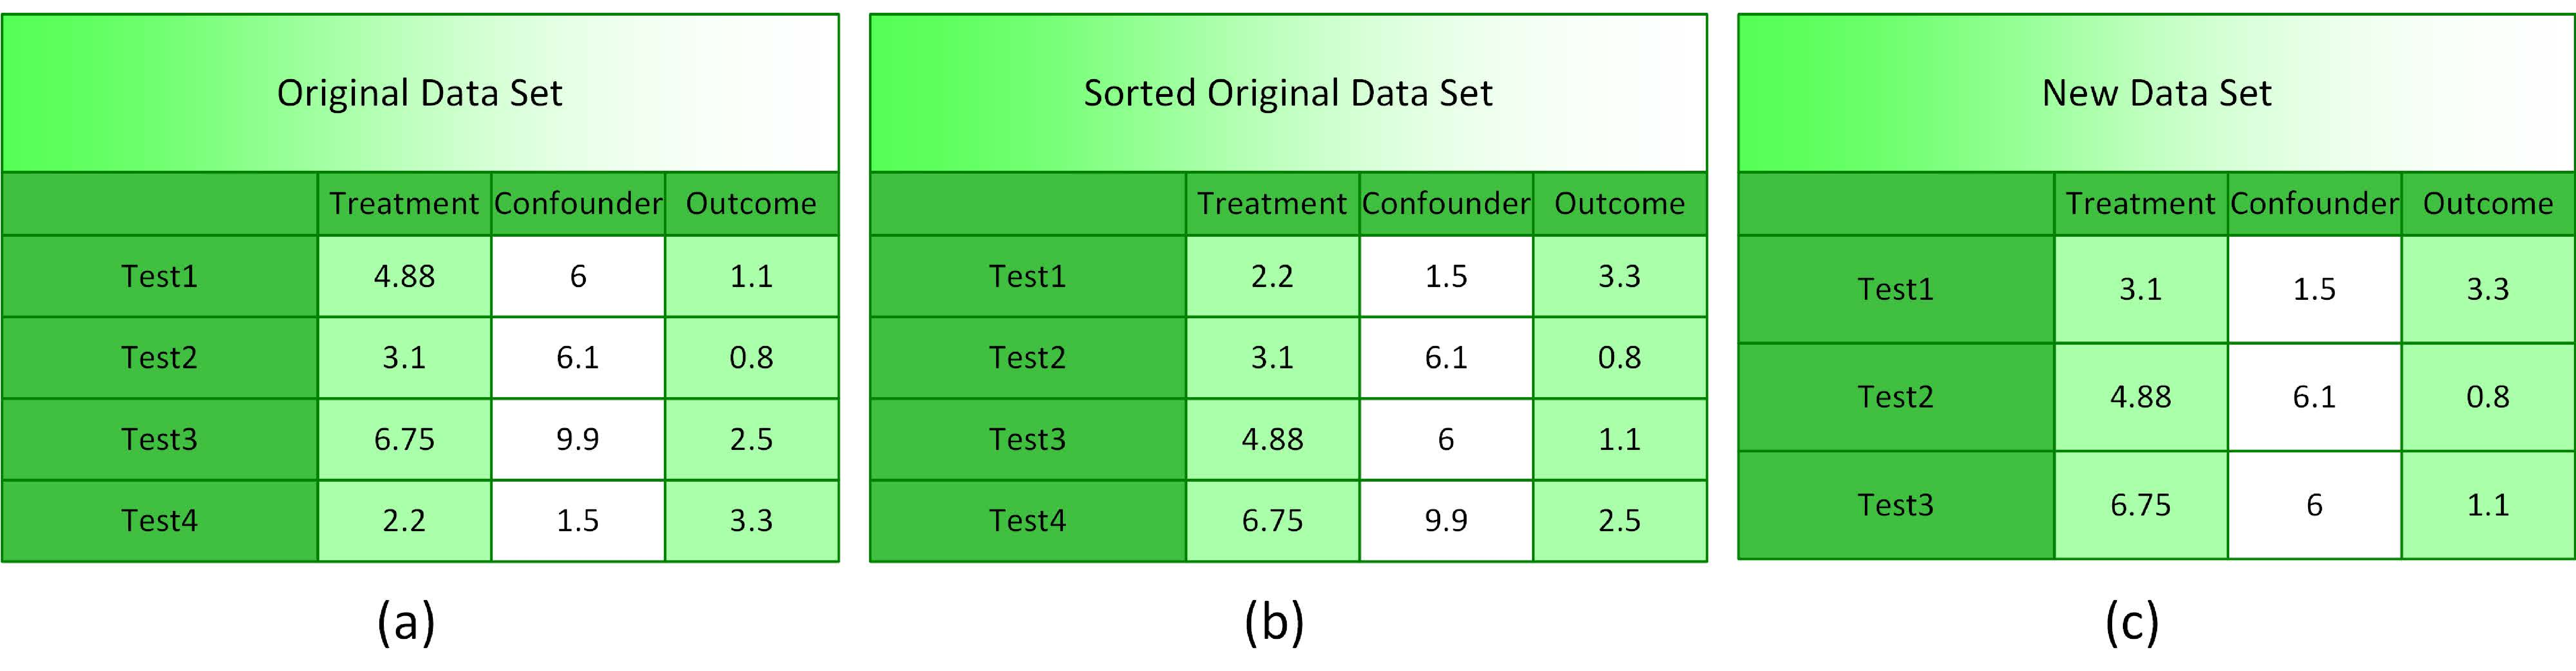
\includegraphics[width=1\textwidth]{chapter4_BART_ACE.pdf}
\caption{EXAMPLE OF TREATMENT VARIABLE INCREAMENT}
\label{bartace}
\end{figure*}

\section{EMPIRICAL EVALUATION}\label{BARTevaluation}% result

To evaluate the effectiveness of BART model, we conducted the empirical study on the same subject programs as described in chapter 3.  The tests suite is also identical to the tests suite in section \ref{numfl_evaluation}.  Overall 92 faulty subject-programs versions with single fault and 25 faulty subject-program versions with two faults. Ochiai, Dstar, SOBER, ESP-SIV and ESP-SCP are used as the base line techniques to be compared with BART model. We also compare the performance of BART model with NUMFL-GPS and NUMFL-CBPS which are the proposed in chapter 3. We measured the costs of applying BART and the other metrics by the percentage of {\it subexpressions} that need to be examined, in decreasing order of suspiciousness scores, to find the fault, assuming the fault is recognized when it is encountered.

In the experiment, we use R package "BARTMachine" \cite{BARTMachine} to fit the BART model. We tried 10 trees and 50 trees in the sum of trees structure.  The BART model is fitted with both passing and failing tests. The number tests for each subject program is from 3000 to 8000 which shown in table \ref{subpro}. We also try to train BART model with fewer data(300 tests). the sensitivity of the BART model to the number of trees and the number of tests are discussed in section \ref{BARTsensitivity}.

\subsection{Comparative Performance of BART vs. Baselines}

Figure \ref{BART_VS_Base} shows the results of comparisons of BART with each of the baseline metrics.  In each graph, the vertical axis represents the percentage improvement (reduction) in cost. The horizontal-axis represents different subject-program versions for which there are cost differences between the metrics, with each version represented by a vertical bar.   Bars above the zero-line represent versions for which BART performed better than the baseline metric and bars below zero represent versions for which BART performed worse.  The length of each bar represents the magnitude of the corresponding cost difference.

\textit{\textbf{ BART vs. Ochiai.}}  Over all 92 faulty subject-program versions, BART performed better than the Ochiai metric on 75 versions but BART performed worse on 17 versions.  There were 41 versions for which BART performed at least 20\% better than the Ochiai metric.  There were just 4 versions for which the latter performed better than BART.

\textit{\textbf{ BART vs. DStar.}}  BART performed better than DStar on 77 subject-program versions but BART performed worse than DStar on 15 versions.  BART performed at least 20\% better than DStar on 44 versions, whereas DStar performed at least 20\% better than BART on just 4 versions.

\textit{\textbf{ BART vs. ESP-SIV.}} BART performed better than ESP-SIV on 78 subject-program versions but BART performed worse than ESP-SIV on 14 versions.  BART performed at least 20\% better than ESP-SIV on 30 versions, whereas ESP-SIV never performed at least 20\% better than BART.

\textit{\textbf{ BART vs. ESP-SCP.}}  BART performed better than ESP-SCP on 75 subject-program versions but BART performed worse than ESP-SCP on 17 versions.  BART performed at least 20\% better than ESP-SIV on 22 versions, whereas ESP-SCP performed at least 20\% better than BART on just 2 versions.

\textit{\textbf{ BART vs. SOBER.}}  BART performed better than SOBER on 73 subject-program versions but BART performed worse than SOBER on 19 versions.  BART performed at least 20\% better than SOBER on 39 versions, whereas SOBER performed at least 20\% better than BART on just 5 versions.

\begin{sidewaysfigure}
\centering
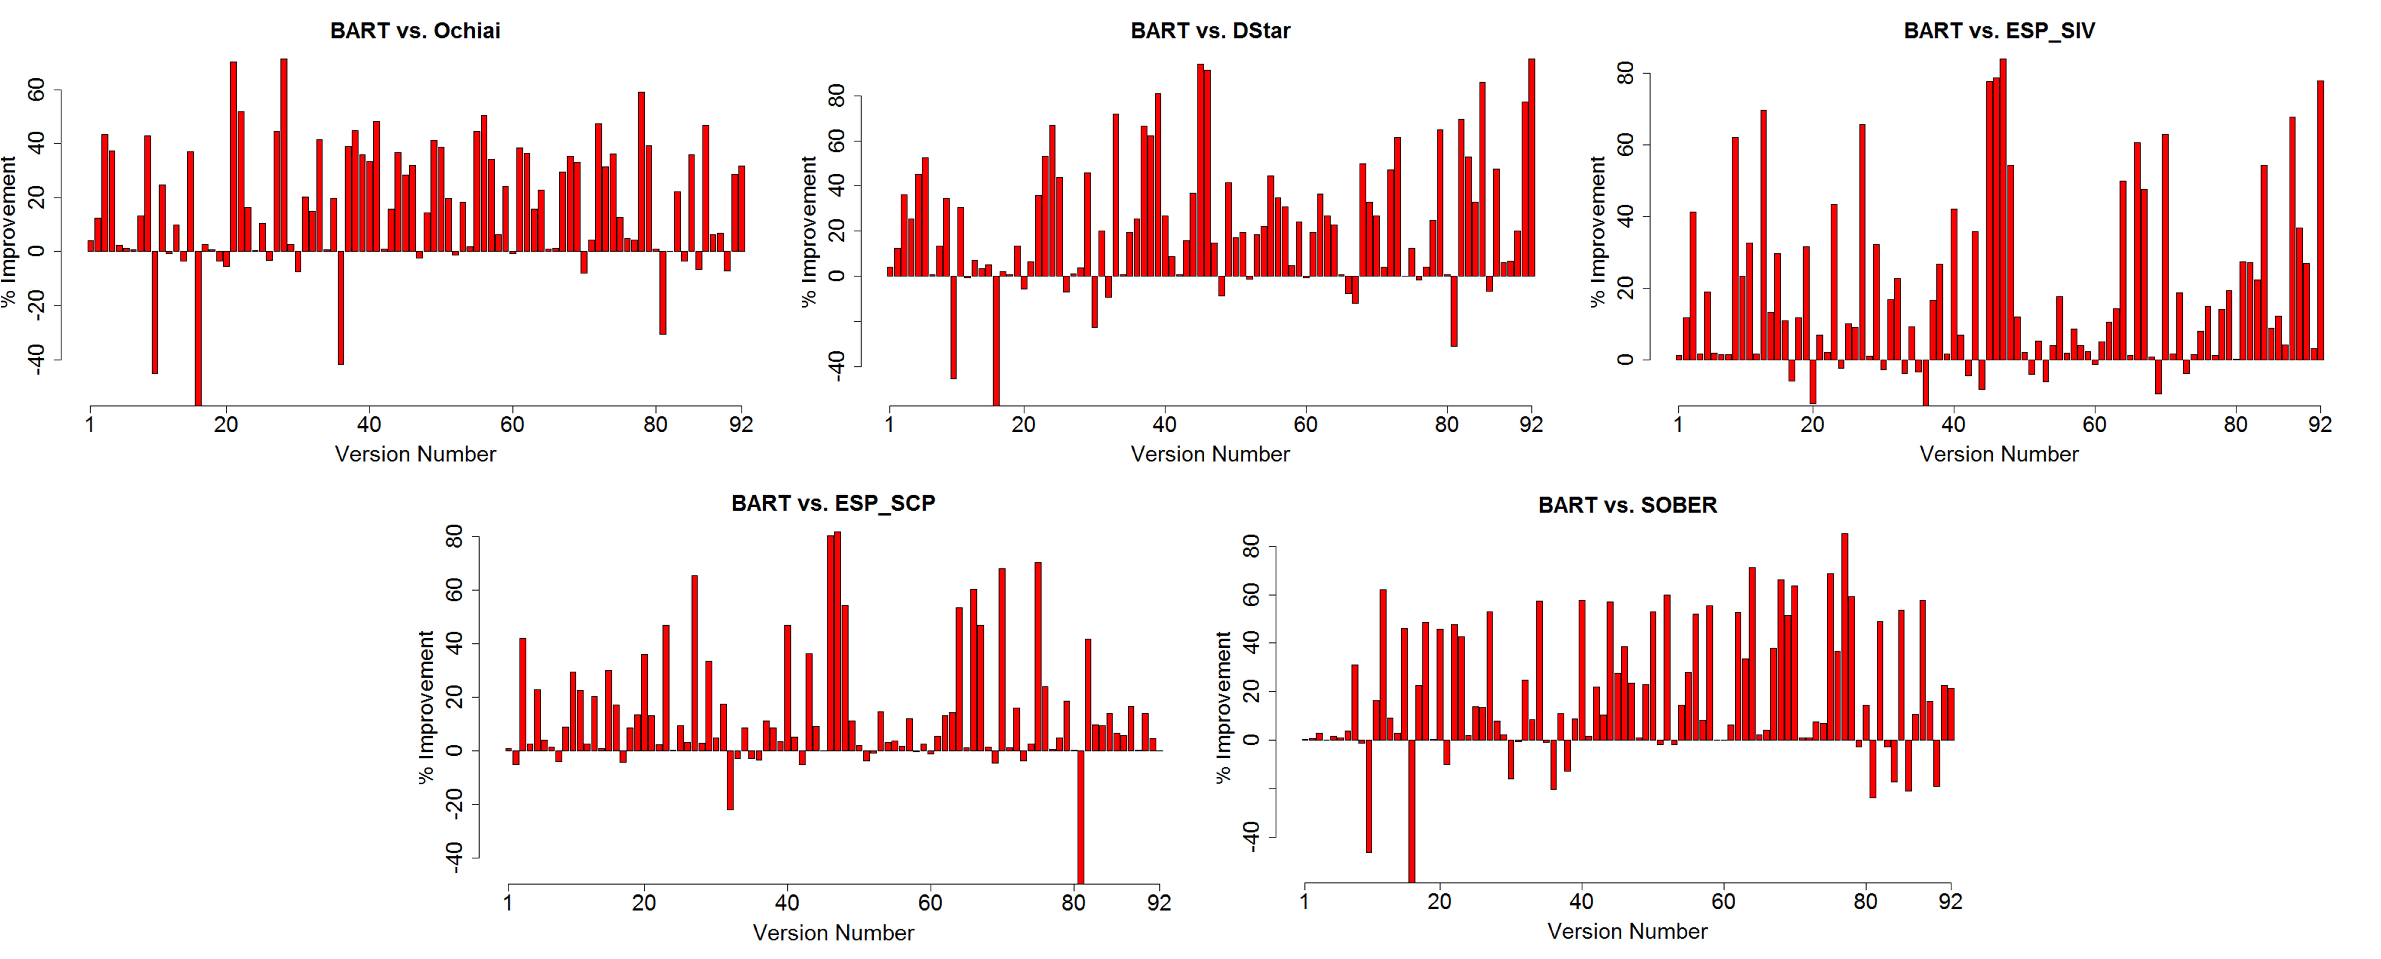
\includegraphics[width=\textwidth]{chapter4_BART_VS_Base.pdf}
\caption{Performance of BART relative to baseline metrics on individual single-fault program versions.}
\label{BART_VS_Base}
\end{sidewaysfigure}

Figure \ref{BART_VS_Base_M} contrasts the performance of BART on the individual two-fault program versions with that of the baseline metrics.  Over all 25 faulty subject-program versions, BART performed better than SOBER on 19 versions but performed worse on 6 versions.  There were 8 versions for which BART performed at least 10\% better than SOBER but 3 versions for which SOBER performed at least 10\% better than BART.  Ochiai performed better than BART on 5 versions but performed worse on 20 versions. BART performed at least 10\% better than Ochiai on 13 versions. BART performed better than both ESP-SIV and ESP-SCP on 20 versions.   BART performed better than DStar on 19 versions.

\begin{sidewaysfigure}
\centering
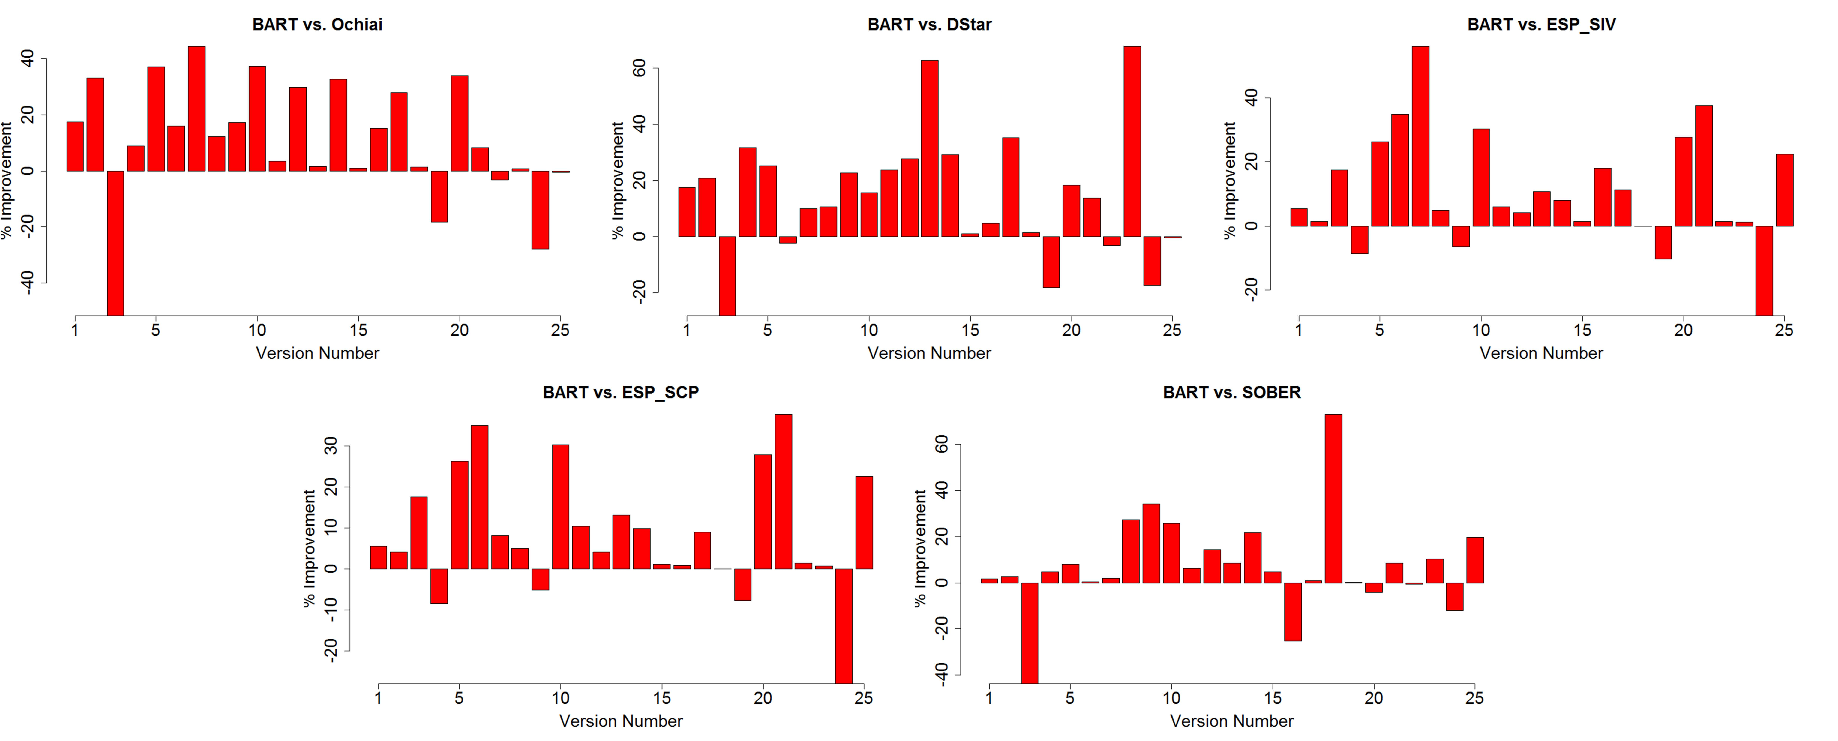
\includegraphics[width=\textwidth]{chapter4_BARTvsBase_M.pdf}
\caption{Performance of BART relative to baseline metrics on individual single-fault program versions.}
\label{BART_VS_Base_M}
\end{sidewaysfigure}


\subsection{BART model vs NUMFL}
Table \ref{tableBARTvsNUMFL} shows the average percentage of subexpressions that had to be examined to find the fault, computed across all the faulty versions, for BART model and NUMFL.  Because QRM is proved to have better performance than DLRM in chapter 3, here we only show the results of NUMFL-GPS-QRM and NUMFL-CBPS-QRM.  From Table \ref{tableBARTvsNUMFL}, there were 11 subject programs for which BART performed better than NUMFL-GPS-QRM. There were 5 subject programs for which NUMFL-GPS-QRM performed better than BART. BART performed better than NUMFL-CBPS-QRM on 14 subject programs. There were only 2 subject programs for which NUMFL-CBPS-QRM performed better than BART.

Figure \ref{BARTvsQRM} graphically contrasts the performance of BART and NUMFL-GPS-QRM on the single fault versions.  BART performed better than NUMFL-GPS-QRM on 54 versions, while NUMFL-GPS-QRM performed better on 38 versions.  BART performed at least 20\% better than NUMFL-GPS-QRM on 9 versions, whereas NUMFL-GPS-QRM performed at least 20\% better than BART on 6 versions. Figure \ref{BARTvsCBPS} graphically contrast the performance of BART and NUMFL-CBPS-QRM on the single fault versions.  BART performed better than NUMFL-CBPS-QRM on 61 versions, while NUMFL-CBPS-QRM performed better on 31 versions.  BART performed at least 20\% better than NUMFL-CBPS-QRM on 17 versions, whereas NUMFL-CBPS-QRM performed at least 20\% better than BART on just 4 versions.

In summary, BART  performed better than both NUMFL-GPS-QRM and NUMFL-CBPS-QRM on single-fault programs. This means that BART model can well approximate the DRF of treatment variable and confounding variables.

\begin{table*}[htbp!]
\caption{AVERAGE FAULT LOCALIZATION COSTS OF BART AND NUMFL METRICS ON SINGLE-FAULT PROGRAM VERSIONS}
\label{tableBARTvsNUMFL}
\centering
      \begin{tabular}{|l|c|c|c|}
      \hline
\multirow{2}{*}{Subject Program}	& \multirow{2}{*}{BART}&	\multicolumn{2}{|c|}{{\bf NUMFL}}	\\	\cline{3-4}
& & GPS-QRM	&CBPS-QRM \\ \hline
Apache\_EigenDecompose &	2.50\%&	12.3\%	&	8.8\%	\\	\hline
Apache\_DScompiler&	9.72\%&	11\%	&	12\%	\\	\hline
Apache\_BigMatrix	&	9.00\%&11.4\%	&	9.9\%	\\	\hline
Apache\_Rotation3D&	9.07\%&	8\%	&	18.9\%	\\	\hline
Ojaljo\_SchurDecompose&	10.61\%&	11.4\%	&	14\%	\\	\hline
Jama\_MatrixDecompose	&11.62\%&	14.2\%	&	23\%	\\	\hline
SciMark\_LU&8.33	\%&	15.3\%	&	27.8\%	\\	\hline
SciMart\_FFT&	 27.59\%&	9.5\%	&	19.8\%	\\	\hline
Apache\_SymmLQ&	 1.75\%&	2.6\%	&	4.4\%	\\	\hline
Apache\_SplineInterpolator&	 37.78\%&	31.7\%	&	35\%	\\	\hline
Apche\_SimpleRegress&	 1.70\%&	4.3\%	&	17\%	\\	\hline
Apache\_SchurTransformer&	 4.56\%&	3.3\%	&	14.9\%	\\	\hline
Apache\_MillerUpdatRegress&	 1.24\%&	7.5\%	&	9.9\%	\\	\hline
Apache\_HarmonicFitter&	30.10\%&	27.3\%	&	32\%	\\	\hline
Apache\_FastSine&	1.53\%&	1.5\%	&	13\%	\\	\hline
Apache\_FastCosine	&1.29	\%&1.3\%	&	1.2\%	\\	\hline
Average Cost	&	10.52\%&10.8\%	&	16.4\%	\\	\hline
\end{tabular}
\end{table*}

\begin{figure*}[!thpb]
\centering
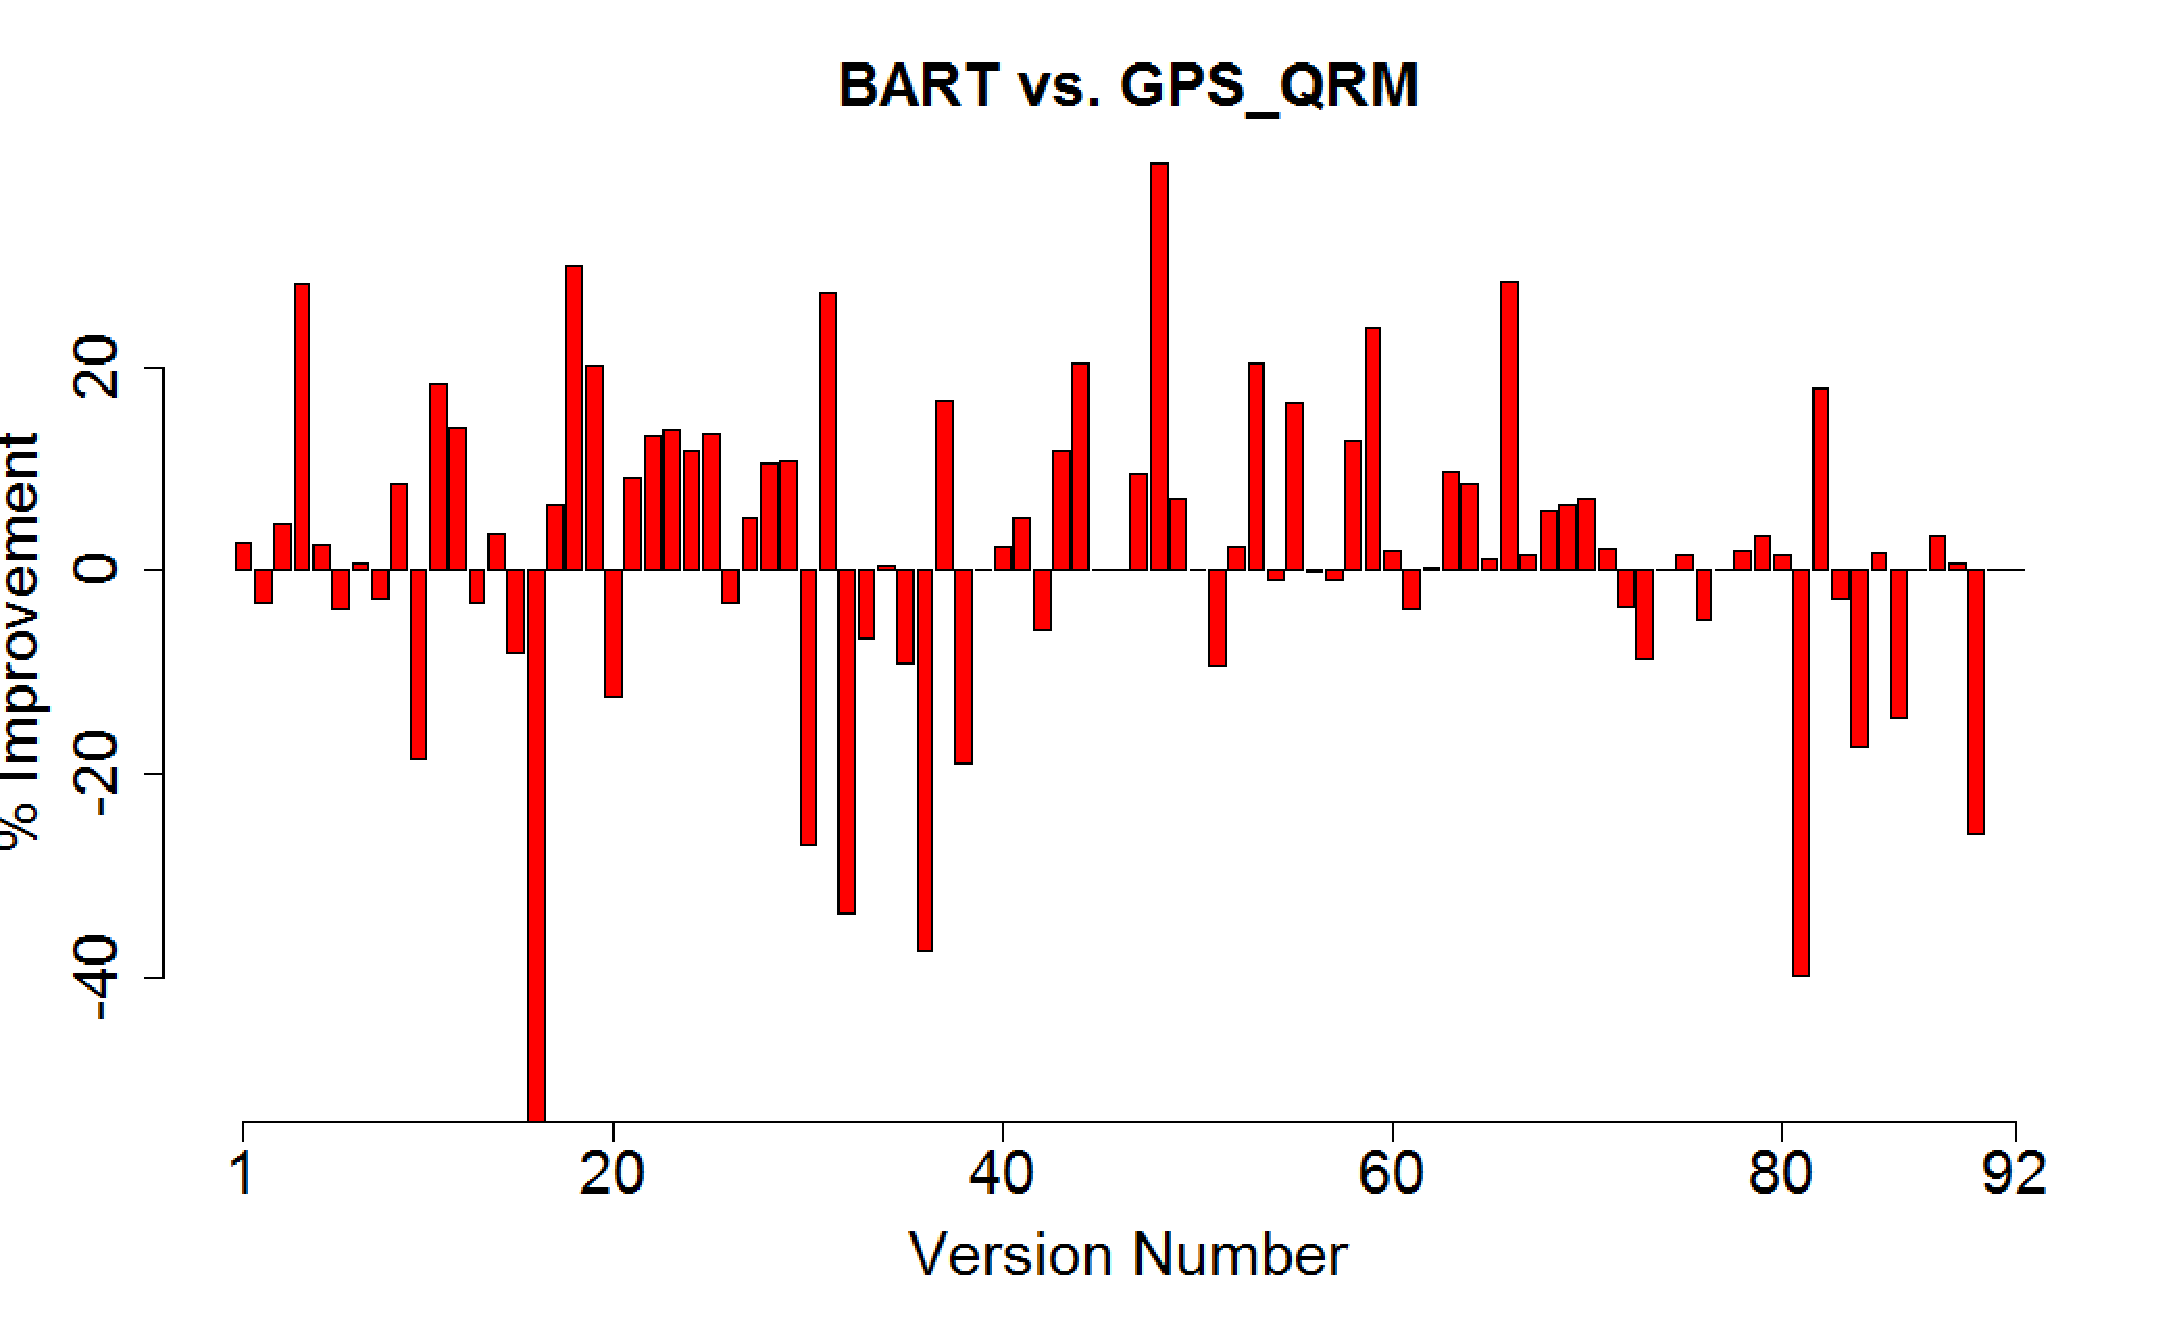
\includegraphics[width=0.8\textwidth]{chapter4_BARTvsGPS_QRM.pdf}
\caption{Relative performance of NUMFL-GPS-QRM with and without data from passing runs, on individual single-fault program versions.}
\label{BARTvsQRM}
\end{figure*}

\begin{figure*}[!thpb]
\centering
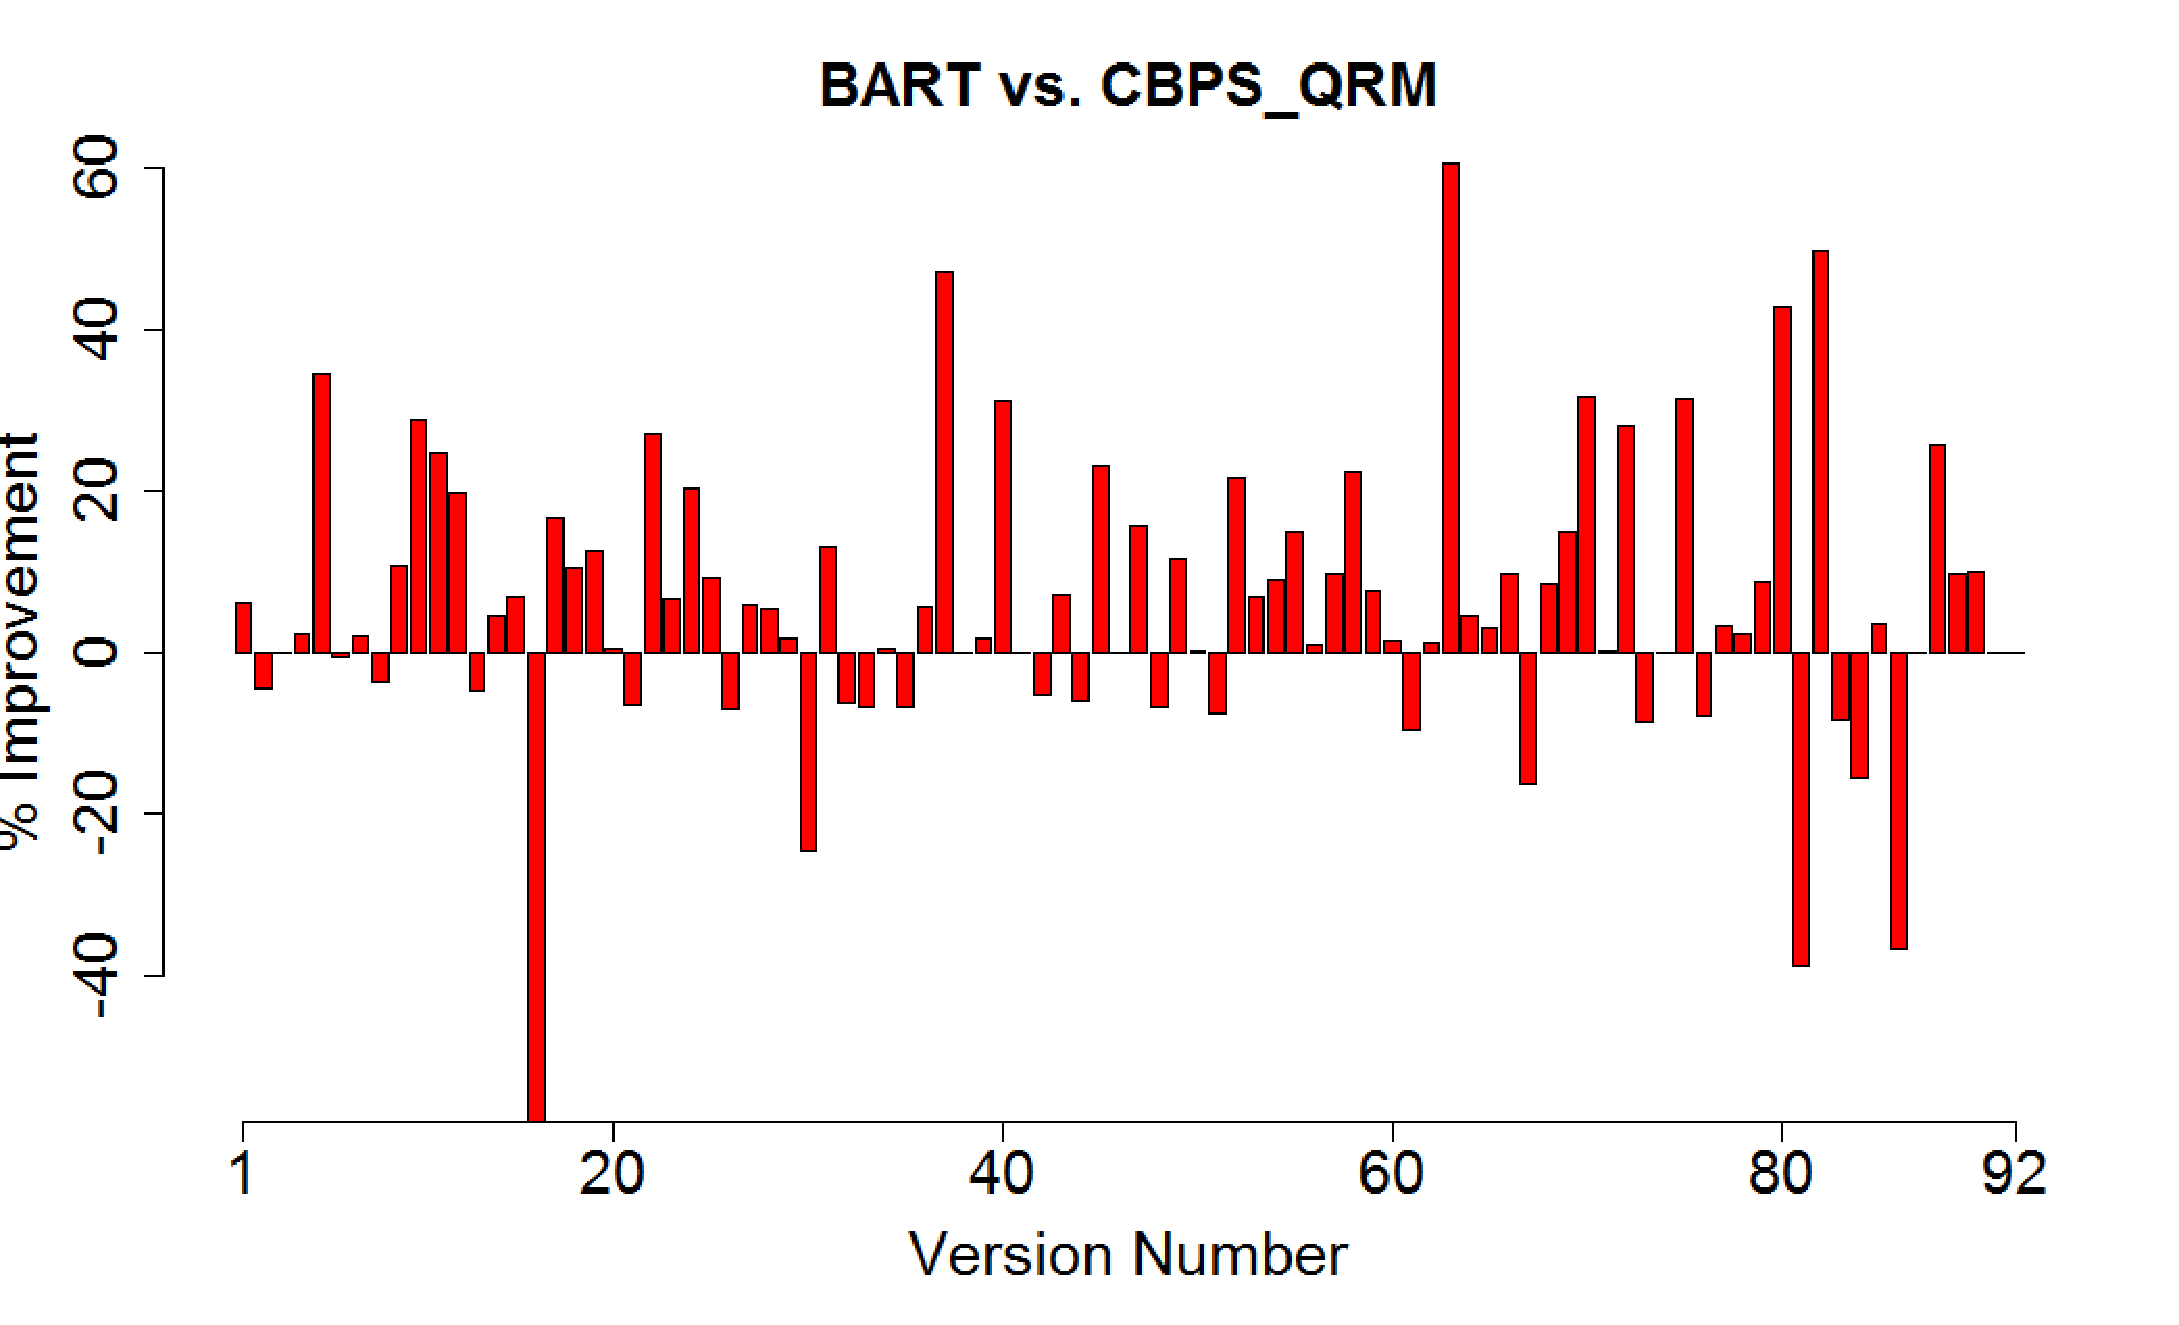
\includegraphics[width=0.8\textwidth]{chapter4_BARTvsCBPS.pdf}
\caption{Relative performance of NUMFL-GPS-QRM with and without data from passing runs, on individual single-fault program versions.}
\label{BARTvsCBPS}
\end{figure*}

Table \ref{tableBARTvsNUMFL_M} shows the average cost, over the faulty versions of each subject program into which two faults were injected, of localizing the first fault to be found, for both BART and NUMFL.  From Table \ref{tableBARTvsNUMFL_M}, BART and NUMFL-GPS-QRM have similar performance on two faults subject programs. BART performed better than NUMFL-GPS-QRM on the versions of  2 subject programs, but performed worse than NUMFL-GPS-QRM on the versions of 3 subject program.  BART performed better than NUMFL-CBPS-QRM on the versions of 4 subject programs, but performed worse than NUMFL-CBPS-QRM on the versions of only 1 subject program.

Figure \ref{BARTvsGPS_M} graphically contrasts the performance of the BART and NUMFL-GPS-QRM on the individual two-fault versions.  BART performed better than NUMFL-CBPS-QRM on 13 versions and NUMFL-GPS-QRM performed worse on 12 versions.  BART performed at least 10\% better than NUMFL-GPS-QRM on 7 versions, whereas NUMFL-CBPS-QRM performed at least 10\% better than NUMFL-GPS-QRM on just 1 version. Figure \ref{BARTvsCBPS_M} graphically contrasts the performance of the BART and NUMFL-CBPS-QRM on the individual two-fault versions.  BART performed better than NUMFL-CBPS-QRM on 13 versions and NUMFL-CBPS-QRM performed worse on 12 versions.  BART performed at least 10\% better than NUMFL-CBPS-QRM on 7 versions, whereas NUMFL-CBPS-QRM performed at least 10\% better than NUMFL-GPS-QRM on just 1 version.

\begin{table*}[htbp!]
\caption{AVERAGE FAULT LOCALIZATION COSTS OF BART AND NUMFL ON MULTIPLE-FAULT PROGRAM VERSIONS}
\label{tableBARTvsNUMFL_M}
\centering
      \begin{tabular}{|l|c|c|c|}
      \hline
\multirow{2}{*}{Subject Program}	& \multirow{2}{*}{BART}&	\multicolumn{2}{|c|}{{\bf NUMFL}}	\\	\cline{3-4}
& & GPS-QRM	&CBPS-QRM \\ \hline
Apache\_EigenDecompose	&7.98	\%&10.3\%	&	11.1\%	\\	\hline
Apache\_DScompiler	&	5.13\%&4.5\%	&	5.9\%	\\	\hline
Apache\_Rotation3D	&	10.69\%&7.0\%	&	3.0\%	\\	\hline
Ojaljo\_SchurDecompose	&17.55	\%&5.4\%	&	19.8\%	\\	\hline
Jama\_MatrixDecompose	&	4.65\%&14.1\%	&	23.4\%	\\	\hline
{\bf Average Cost} &9.20\% &8.26\% &12.64\%\\ \hline
\end{tabular}
\end{table*}

\begin{figure*}[!thpb]
\centering
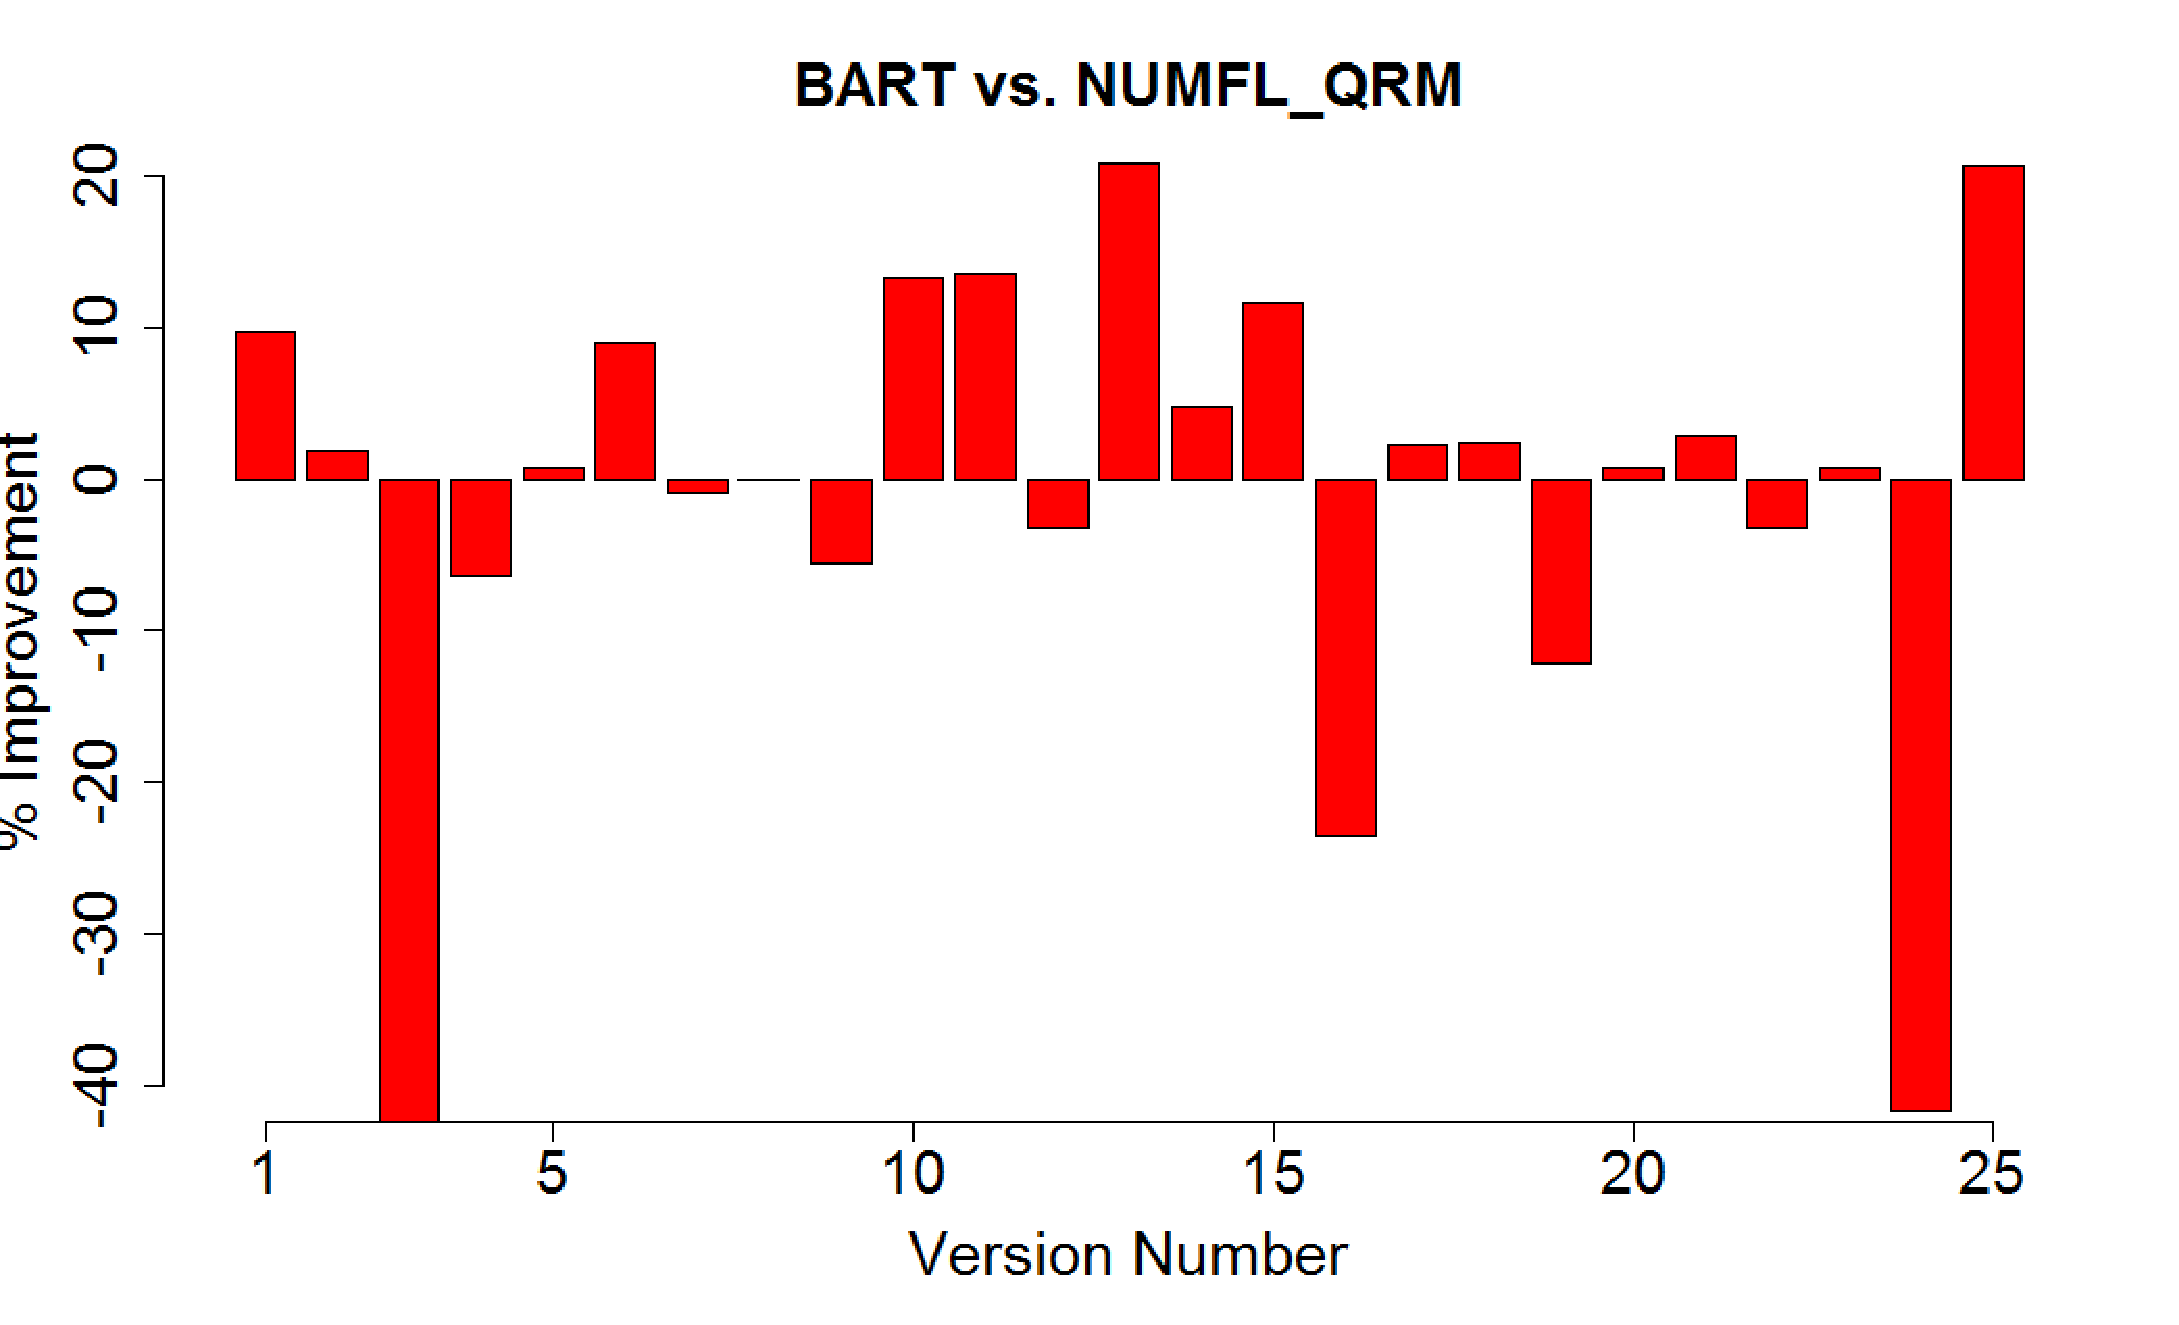
\includegraphics[width=0.8\textwidth]{chapter4_BARTvsGPS_QRM_M.pdf}
\caption{Relative performance of NUMFL-GPS-QRM with and without data from passing runs, on individual single-fault program versions.}
\label{BARTvsGPS_M}
\end{figure*}

\begin{figure*}[!thpb]
\centering
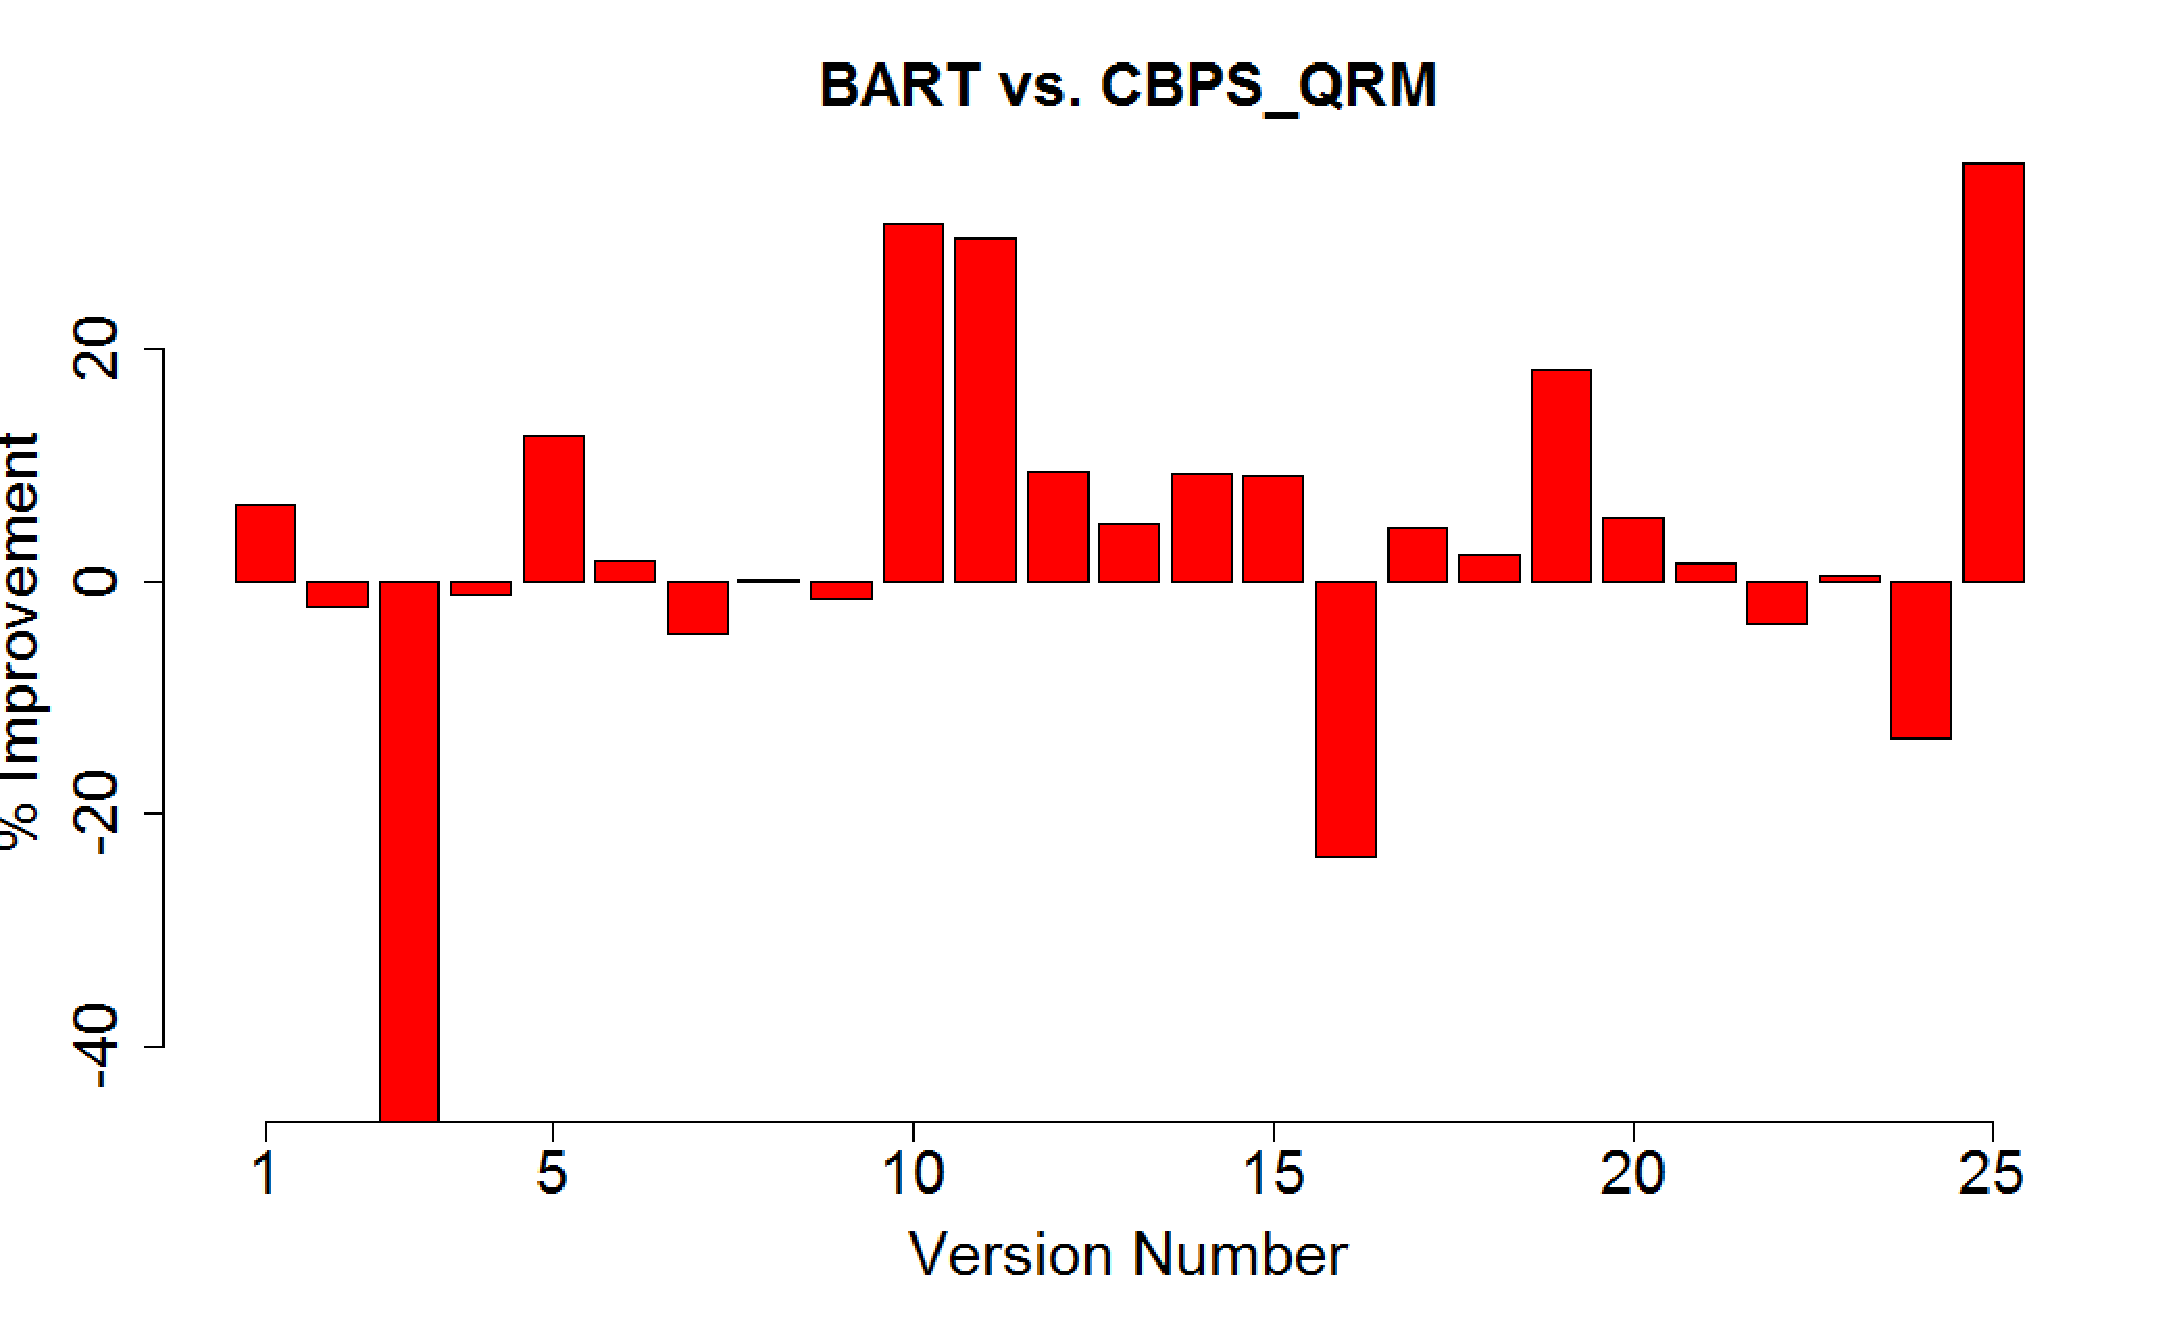
\includegraphics[width=0.8\textwidth]{chapter4_BARTvsCBPS_M.pdf}
\caption{Relative performance of NUMFL-GPS-QRM with and without data from passing runs, on individual single-fault program versions.}
\label{BARTvsCBPS_M}
\end{figure*}

\subsection{Sensitivity of BART model on the number of trees and number of tests}\label{BARTsensitivity}

In previous sections, we use the full observational data of tests to fit a BART model with 10 trees in the sum of trees structure. In this section, we will analyze if increasing number of trees or decreasing the number of tests would influence the performance of BART. In Table \ref{sensitivity}, the first column of numbers is the fault localization cost of BART model contains 10 trees and fitted with full observational data (3000-8000 tests). The second column of numbers is the fault localization cost of BART model contains 50 trees and fitted with full observational data. The third column of numbers is the fault localization cost of BART model contains 10 trees but fitted with only 300 tests' data. From Table \ref{sensitivity}, when increased the number of trees from 10 to 50, BART model has better performance on 6 subject programs. But there are also 6 subject program where BART model's performance become worse after increasing the number of trees. The average cost across 16 subject programs is roughly same: 10.52\% for BART model with 10 trees and 10.58\% for BART model with 50 trees. This means that 10 trees are enough to handle the nonlinearity problem in AFCE estimation.  When we decrease the number of tests to 300, the average cost is slightly increased to 10.74\%.  This means that BART model does not require a large number of tests to localize faults in numerical softwares.

\begin{table*}[htbp!]
\caption{AVERAGE FAULT LOCALIZATION COSTS OF BART MODEL WITH DIFFERENT NUMBER OF TREES AND TESTS ON ONE SINGLE-FAULT PROGRAM VERSIONS }
\label{sensitivity}
\centering
      \begin{tabular}{|l|c|c|c|}
      \hline
\multirow{2}{*}{{\bf Subject Program}}	&	\multicolumn{3}{|c|}{{\bf BART Model}}	\\	\cline{2-4}
& 10 trees & 50 trees & 300 tests\\ \hline
Apache\_EigenDecompose			&	2.50	\%	&	3.07	\%	&	2.38	\%	\\ \hline
Apache\_DScompiler			&	9.72	\%	&	8.61	\%	&	9.64	\%	\\ \hline
Apache\_BigMatrix			&	9.00	\%	&	9.05	\%	&	9.00	\%	\\ \hline
Apache\_Rotation3D			&	9.07	\%	&	8.73	\%	&	8.16	\%	\\ \hline
Ojaljo\_SchurDecompose			&	10.61	\%	&	9.89	\%	&	11.44	\%	\\ \hline
Jama\_MatrixDecompose			&	11.62	\%	&	11.16	\%	&	11.32	\%	\\ \hline
SciMark\_LU			&	8.33 \%	&	9.72	\%	&	6.94	\%	\\ \hline
SciMart\_FFT			&	27.59	\%	&	26.72	\%	&	27.59	\%	\\ \hline
Apache\_SymmLQ			&	1.75	\%	&	1.75	\%	&	1.75	\%	\\ \hline
Apache\_SplineInterpolator			&	37.78	\%	&	40	\%	&	45.56	\%	\\ \hline
Apche\_SimpleRegress			&	1.70	\%	&	1.70	\%	&	1.70	\%	\\ \hline
Apache\_SchurTransformer			&	4.56	\%	&	4.88	\%	&	4.23	\%	\\ \hline
Apache\_MillerUpdatRegress			&	1.24	\%	&	1.24	\%	&	1.24	\%	\\ \hline
Apache\_HarmonicFitter			&	30.10	\%	&	30.08	\%	&	28.06	\%	\\ \hline
Apache\_FastSine			&	1.53	\%	&	1.53	\%	&	1.53	\%	\\ \hline
Apache\_FastCosine			&	1.29	\%	&	1.29	\%	&	1.29	\%	\\ \hline
Average Cost 	&	10.52\% 	&10.58\% 	&10.74\%	\\ \hline
\end{tabular}
\end{table*}

\subsection{Computation Time Analysis}
In this study, we use a Dell Precision T5600 with two 2.30 GHz intel Xeon CPUs and 64 GB RAM. Table \ref{BARTcomputetime} summarized the average computation time of the three BART models described in last section on each subject program.  When the number of trees increased from 10 to 50, the average computation cost nearly doubled. If we reduced number the tests from more than 3000 to 300, the computation cost will reduced more than 50\%.  From Table \ref{BARTcomputetime} and Table \ref{sensitivity}, we can conclude that the BART model with 10 trees and fitted with 300 tests get the best cost-performance ratio among the three BART models fitted with different settings. But we also need to point out that even the BART model is fitted with 300 tests, its computation cost is still about twice of the computation cost of NUMFL. Thus, the computation cost is a weakness of applying BART on localizing faults in numerical softwares. 

\begin{table*}[htbp!]
\caption{AVERAGE COMPUTATION TIME OF NUMFL-GPS-QRM AND NUMFL-CBPS-QRM ON ONE SINGLE-FAULT PROGRAM VERSIONS }
\label{BARTcomputetime}
\centering
      \begin{tabular}{|l|c|c|c|}
      \hline
\multirow{2}{*}{{\bf Subject Program}}	&	\multicolumn{3}{|c|}{Average Computation Time (Secs)}	\\	\cline{2-4}
& 10 trees & 50 trees & 300 tests\\ \hline

Apache\_EigenDecompose	&	2856.73	&	5530.20	&	1205.97	\\ \hline
Apache\_DScompiler	&	628.31	&	1243.78	&	274.88	\\ \hline
Apache\_BigMatrix	&	696.58	&	1337.73	&	292.28	\\ \hline
Apache\_Rotation3D	&	2668.41	&	5550.45	&	1082.64	\\ \hline
Ojaljo\_SchurDecompose	&	2636.96	&	5013.37	&	1313.53	\\ \hline
Jama\_MatrixDecompose	&	3134.49	&	6005.71	&	1262.88	\\ \hline
SciMark\_LU	&	167.94	&	332.45	&	121.38	\\ \hline
SciMart\_FFT	&	393.26	&	842.31	&	234.09	\\ \hline
Apache\_SymmLQ	&	908.12	&	1986.32	&	245.21	\\ \hline
Apache\_SplineInterpolator	&	364.80	&	747.42	&	135.00	\\ \hline
Apche\_SimpleRegress	&	823.34	&	1685.88	&	227.27	\\ \hline
Apache\_SchurTransformer	&	768.44	&	1539.44	&	315.65	\\ \hline
Apache\_MillerUpdatRegress	&	396.10	&	808.59	&	198.61	\\ \hline
Apache\_HarmonicFitter	&	326.09	&	673.73	&	120.28	\\ \hline
Apache\_FastSine	&	1006.86	&	2064.98	&	259.78	\\ \hline
Apache\_FastCosine	&	1089.13	&	2229.39	&	294.56	\\ \hline
\end{tabular}
\end{table*}

\section{RELATED WORK}\label{BARTrelatedwork}
The most related works to this study are those using BART model to estimate treatment causal effect. Hill et al. proposed to apply BART model for causal inference and data science \cite{hill2012bayesian, hill2013assessing}. In the paper, they designed the method of using BART to estimate average causal effect of binary treatment variable and discussed how to use BART to handle continuous treatment variables and outcome missing data. Later, Green et al. applied BART to model heterogeneous treatment effects \cite{green2012modeling}. Sparapani et al. extends the usefulness of BART in medical applications by addressing needs arising in survival analysis \cite{sparapani2016nonparametric}.

Another related work is using tree structure in fault localization. Chen et al \cite{chen2004failure} present a decision tree learning approach to identify the causes of failures in internet sites. Francis et al \cite{francis2004tree} use tree based method to classify software failures. Kiciman et al \cite{kiciman2005root} use decision tree to diagnose which component of large scale systems is the root cause of failure. However, unlike our models, all their works do not localize the fault on statement level.

\section{CONCLUSION}\label{BARTconclusion}
BART model is a Bayesian non-parametric model which can capture both nonlinearities and interactions between variables without knowing the information about how these variables are parametrically related . BART uses a sum of trees structure to approximate the dose response function of continuous treatment variables. The AFCE can be estimated by averaging the causal effect of treatment on outcome at each observation unit. We reported the result of an empirical comparison of BART model to several competing fault localization metrics on both single-fault subject programs and multiple-fault subject programs. BART model performed significantly better than the other techniques. We also compare the BART model with NUMFL, which is introduced in chapter 3. The result shows BART model outperforms NUMFL on single faults localization. In multiple faults localization, BART and NUMFL has similar performances.  We also study the sensitivity of the BART model to the number of trees and the number of tests. The result shows BART is robust on the sample size and number of trees.   